\documentclass[twoside]{oss-conf}
\usepackage{lmodern}
\usepackage{cmap}
\usepackage[english,slovak]{babel}             % use english and your language respectively ... czech, polish, ...
\usepackage[T1]{fontenc}
\usepackage[utf8]{inputenc}                    % use only UTF-8 encoding 
\usepackage{amsmath}
\usepackage{amscd,amssymb,amsfonts}
\usepackage[sort,nocompress]{cite} 
\usepackage{graphicx}                          % use for include pictures *.jpg, *.png, *.pdf
  %\usepackage{color}
  %\usepackage{colortbl}
  %\usepackage{multicol}
  %\usepackage{comment}
\usepackage{fancyhdr}
\usepackage[pdftex,unicode,bookmarks=false]{hyperref}  % for e-mail and url adress
\usepackage{eurosym}
\usepackage{listings}



%.............................................................................
\begin{document}

%..................................................................................
\setcounter{page}{1}                            % číslo prvej stránky príspevku
\def\volumeDOI{OSSConf 2012:\  }                % číslo zborníka
\def\konfera{Konferencia OSSConf 2012}

\pagestyle{fancy}
\fancyfoot{}\fancyhead[LE,RO]{\thepage}\fancyhead[LO]{\nouppercase{\leftmark: \rightmark}}\fancyhead[RE]{\nouppercase{\konfera}}



%........................................................................................................................................
%     TU ZAČÍNA PÍSAŤ AUTOR
%........................................................................................................................................


	

%.............................................. pre slovenčinu
\def\solutionname{Riešenie}
\def\addressS{Kontaktná adresa}
\def\addressSis{Kontaktné adresy}
\def\rbCurrentaddress{Aktuálna adresa}
\def\rbEmailaddress{E-mailová adresa}
\def\keywordsnameS{Kľúčové slová}     
%.............................................. pre češtinu odpoznámkovať
%\def\solutionname{Řešení}
%\def\addressS{Kontaktní adresa}
%\def\addressSis{Kontaktní adresy}
%\def\rbCurrentaddress{Aktuální adresa}
%\def\rbEmailaddress{E-mailová adresa}
%\def\keywordsnameS{Klíčová slova}


%%.............................................. slovenský alebo český názov
% pre kratšie názvy  použi iba príkaz   \title{CELÝ NÁZOV ČLÁNKU}  
\title[Multitasking pre ARM]{Preemptívny multitasking\\ pre mikrokontroléry s jadrom arm cortex m3} 


%.............................................. anglický názov
\titleA[Multitasking for ARM]{Preemptive multitasking\\ for arm cortex m3 core microcontrollers}


%.............................................. autori (jeden alebo viac) .. každý podľa vzoru:
 \author[M. Chovanec]{Michal Chovanec}{Bc.}{}{SK}
 \address{}
% \curraddress{alternatívna adresa}
 \emailh{Michal.Chovanec@st.fri.uniza.sk}
 \urladdressh{}

%.............................................. kľúčové slová slovensky/anglicky
\keywords{multitasking, operačný systém, arm cortex}
\keywordsA{multitasking, operating system, arm cortex}


%.............................................. slovenský abstrakt
\selectlanguage{slovak}

\begin{abstract}
Článok popisuje realizáciu preemptivného multitaskingu využitom v experimentálnom operačnom systéme pre mikrokontrolér s jadrom ARM Cortex M3. Vývoj je realizovaný za použitia OSS nástrojov,  OS Linux, kompilátor gcc a samotný program na nahratie, stlink. 
\end{abstract}


%.............................................. anglický abstrakt
\selectlanguage{english}

\begin{abstractA}
The article describes the implementation of preemptive multitasking in the experimental operating system for microcontrollers with ARM Cortex M3 core. The development is realized using OSS tools, Linux, gcc compiler and the program to load, stlink.
\end{abstractA}



\selectlanguage{slovak}
%.............................................. moje makrá
\newtheorem{theorem}{Veta}[section]
\newtheorem{corollary}[theorem]{Tvrdenie}
\newtheorem{lemma}[theorem]{Lema}
\newtheorem{exmple}[theorem]{Príklad}
\newtheorem{defn}[theorem]{Definícia}
\newtheorem{rmrk}[theorem]{Poznámka}
            %%% for no-italic, numbered environments, use:
\newenvironment{definition}{\begin{defn}\normalfont}{\end{defn}}
\newenvironment{remark}{\begin{rmrk}\normalfont}{\end{rmrk}}
\newenvironment{example}{\begin{exmple}\normalfont}{\end{exmple}}
            %%% for unnumbered environments, use f.e.
\newtheorem*{remarque}{Poznámka}

\newcommand\dd{\mathop{\rm d\!}\nolimits}
\newcommand\sgn{\mathop{\rm sgn}\nolimits}
\renewcommand{\labelitemi}{$-$}


%.............................................. telo článku
\maketitle

\section*{Úvod}

Zariadenia riadené monolitickým mikropočítačom sa stali súčasťou každodenného života. Nasadenie mikrokontrolérov už nie je len v jednoúčelových zariadeniach, ako sú napr. mikrovlnné rúry, či riadenie motora osobného auta, ale už bežne zasahujú do komplexnejších zariadení. Príkladom zo spotrebnej elektroniky sú napríklad mobilné telefóny, hudobné a DVD prehrávače. V priemysle je to napr. riadenie robotov, zber senzorických dát, či rôzne druhy regulátorov.

	Akonáhle je požiadavka na viacúlohové využitie mikrokontroléra, dostáva použitie operačného systému s multitaskingom mimoriadnu prioritu pri návrhu. Operačné systémy určené pre PC často neprichádzajú do úvahy, zariadenie je limitované najmä RAM pamäťou. Pre experimentálne overenie jednoduchého systému schopného riadiť proces v reálnom čase, bol zvolený mikrokontrolér STM32F100 \cite{stm32f}. Je to dostupný mikrokontrolér, z rady STM32 patrí k menej výkonným a lacným modelom z rodiny ARM. Je ale možné použiť vyššie modely, napr. STM32F103, prípadne siahnuť po výrobkoch Texas Instruments a ich Stellaris mikrokontroléroch \cite{stellaris}.

	Použité jadro CortexM3 predstavuje 32 bitovú architektúru z rodiny ARM. Jadro prebralo mnoho výhodných rysov risc architektúry. Medzi najdôležitejšie prvky zvyšujúce výkon patrí:
\begin{itemize}
	\item množstvo pracovných registrov, 12 + 4
	\item inštrukcie typu load store, minimalizujú prácu s pamäťou
	\item nízky počet inštrukcií
	\item trojstupňová pipeline
	\item pokročilý prerušovací systém
\end{itemize}
	Vykonávanie inštrukcie prebieha v trojstupňovej pipeline – fetch, decode, execute. V kombinácii s nízkym počtom inštrukcií a load store architektúry je možné pomerne jednoducho predvídať aké prostriedky budú vyžadované nasledujúcou inštrukciou. To umožňuje vysoké zvýšenie výkonu, čiastočnú paralelizáciu vykonania inštrukcií a zmenšiť počet tranzistorov na čipe. Problematike architektúry ARM sa venuje \cite{armarch}.

\section{Multitasking}

Myšlienka OS je založená na silnej modularite, minimalizácií časových latencií a rešpektovania malej kapacity pamäte. Dôsledkom  je koncepcia nano kernelu, kde samotný kernel len prepína úlohy a všetko ostatné je realizované formou knižníc, prípadne úloh. 
	Ovládače hardvéru môžu byť realizované ako bežné volania funkcií, alebo formou posielania správ. Vtedy je ovládač založený ako samostatná úloha, čakajúca na správu. Niektoré situácie je vhodné riešiť čisto len použitím správ a riadiť proces udalosťami. Príkladom sú aplikácie, kde je dôraz kladený na spotrebu. V dobe neprítomnosti udalosti môže byť mikroprocesor v režime spánku. Názorná ukážka tejto myšlienky je uvedená v \cite{eventprog}.

	
	Preemptívny multitasking umožňuje prerušiť vykonávaný proces bez jeho aktívnej spolupráce a začať vykonávať ďalší proces. Plánovač cyklicky strieda procesy, napr. podľa priorít a umožňuje zdanlivý beh viacerých procesov súčastne. V prípade operačného systému použitom na mikrokontroléri sa skôr hovorí o vláknach. 
	Celý program je umiestnený vo vnútornej flash pamäti. Pre náročnejšie aplikácie je výhodou umiestniť do flash len zavádzač spolu s jednoduchým monitorovacím programom a pripojiť externú RAM pamäť, do ktorej sa umiestni celý systém, vrátane požadovaných programov.

	Samotná myšlienka realizácie multitaskingu na použitom mikrokontroléri je veľmi jednoduchá. Nevyhnutnou požiadavkou je prítomnosť časovača, ktorý umožňuje vyvolať prerušenie. 
	Vo vyvíjanom operačnom systéme je podľa odporučenia použitý sys tick timer. Ten periodicky vyvoláva prerušovaciu rutinu :

\begin{verbatim}
void SysTick_Handler(void) __attribute__(( naked ));
\end{verbatim}

Následne je nutné uložiť kontext procesora, prepnúť na ďalšiu úlohu, obnoviť kontext a vystúpiť z prerušovacej rutiny. Kontext použitého procesora zahŕňa minimálne hodnoty registrov, programového čítača a stavové registre.


	Spomenuté prepnutie kontextu znázorňuje nasledujúci kúsok programu :

{\small
\begin{verbatim}
void SysTick_Handler(void) 
{ 
 save_context(); 
 
 //prečítanie hodnoty zásobnika
 uint *sp=(uint*)__get_MSP();		

 //uloženie ukazovateľa zásobnika
 if (__current_task__!=SYSTEM_INIT)
  __task__[__current_task__].sp=(uint*)sp; 
 else 
  __current_task__=0;

 //nájdenie ďalšej pripravenej úlohy
 scheduler(); 					

 //nastavenie zásobnika
 sp=__task__[__current_task__].sp;		

 //obnova kontextu a návrat z prerušenia
 restore_context(); 				
}
\end{verbatim}
}
Funkcia scheduler() nastaví novú hodnotu pre premennú current task. Kľúčová myšlienka multitaskingu je existencia viacerých zásobníkov. Pre každú úlohu je prítomný jeden. Rutina ich cyklicky vymieňa a mení hodnotu fyzického ukazovateľa na zásobník. Prerušená úloha sa vďaka tomu môže vrátiť a pokračovať v pôvodnom stave. Samotný hardvér mikrokontroléra automaticky ukladá niektoré registre, to umožňuje minimalizovať čas potrebný na prepnutie kontextu. Uloženie a obnova kontextu je vďaka tomu veľmi jednoduchá :

\begin{verbatim}
#define save_context() __ASM volatile ("push {r4-r12}");
\end{verbatim}
obnova : 
\begin{verbatim}
#define restore_context() 	 
 __ASM volatile ("msr msp, %0\n\t" : : "r" (sp) );
 __ASM volatile ("mvn lr,#6");
 __ASM volatile ("pop {r4-r12}");
 __ASM volatile ("bx lr");
\end{verbatim}


Pre plánovanie ďalšej úlohy bol zvolený round robin algoritmus. Pre malý počet úloh je vyhovujúci. Výhodou je jednoduchosť spojená s rýchlosťou nájdenia ďalšej úlohy a prípadná možnosť implementácie prioritného plánovania. Nasledujúci kúsok programu ukazuje
možnú realizáciu plánovača. Podmienkou je aspoň jedna aktívna úloha, inak sa uvedený program zacyklí v nekonečnej slučke.
Nakoľko je zmyslom operačného systém koordinovať aspoň jednu úlohu je táto podmienka vždy splnená.

\begin{verbatim}
void scheduler()
{
 do
  {
   __current_task__++;
   if (__current_task__>=TASK_MAX_COUNT)
    __current_task__=0;
  }
   while ( ( (__task__[__current_task__].flag&TF_CREATED)==0) );
}
\end{verbatim}

Algoritmus jednoducho prechádza pole potenciálnych úloh a vyberie prvú existujúcu. 
Za povšimnutie stojí realizácia čítača bez funkcie modulo. Je to spôsobené nedostupnosťou inštrukcie delenia na niektorých mikroprocesoroch, kompilátor by potom musel použiť časovo náročnejšie riešenie. Podobné riešenia sú typické pre programovanie malých
mikrokontrolérov.

Pre užívateľa systému je najdôležitejšia funkcia na vytvorenie novej úlohy. Parametrami je ukazovateľ na main funkciu úlohy,
ukazovateľ na zásobník úlohy a jeho veľkosť. Vráti id úlohy ak sa ju podarilo vytvoriť.
\begin{verbatim}
uint create_task(void *task_ptr, uint *s_ptr, uint stack_size)
{
 stack_size/=sizeof(uint);

 u32 task_id=TASK_MAX_COUNT;
 u32 res=TASK_MAX_COUNT;

 do
  {
   task_id--;
   CLI();
   if ((__task__[task_id].flag&TF_CREATED)==TF_NULL)
    {
      init_stack();
     __task__[task_id].flag=TF_CREATED;
     res=task_id;
    }
   SEI();
  }
   while ( (task_id!=0) && (res==TASK_MAX_COUNT) );

 return res;
}
\end{verbatim}

Cyklus prejde zoznam voľných pozícií pre úlohy a prvú voľnú inicializuje pre úlohu. Nevyhnutné je vykonať porovnanie a rezerváciu
atomicky. Z dôvodu prenositeľnosti a modularity systému je atomickosť riešená zákazom a povolením prerušení (CLI() a SEI()).

\section{Vývoj s oss nástrojmi}
Kompilátor gcc pre použitý ARM je možné skompilovať pomocou dostupného skriptu summon-arm-toolchain. Najdôležitejší je ale nástroj stlink, slúžiaci na nahratie skompilovaného binárneho súboru do pamäte mikrokontroléra. Príkaz na nahratie pre mikrokontrolér stm32f100 má nasledujúci tvar :
\begin{verbatim}
~/bin/stlink/flash/st-flash write main.bin 0x8000000
\end{verbatim}
Samotné rozhranie je realizované cez USB s využitím dosky STM 32 Discovery \cite{disckit}. Nahratie prebieha veľmi rýchlo
a ihneď po dokončení začne mikrokontrolér vykonávať program. Existuje možnosť umiestniť program do internej RAM pamäte mikrokontroléra. Túto možnosť je vhodné použiť v štádiu ladenia programu, nakoľko flash pamäť má obmedzený počet prepísaní (výrobcovia udávajú 1000 až 10000).
Pre kompiláciu programu je vhodné vytvoriť makefile, ktorý výrazne urýchli prácu. Výstupom gcc kompilátora je elf súbor. Ten je nutné pomocou objdump prekonvertovať na jednoduchý binárny súbor, bez akejkoľvek hlavičky. Objdump je možné využiť aj na výpis preloženého programu v assembleri. Pri vývoji je to neoceniteľná pomôcka, nakoľko kompilátor môže pri nevhodne nastavených optimalizáciách vytvoriť
nefunkčný kód. Príkladom je nutnosť uviesť volatile pred každou deklaráciou globálnej premennej používanej v prerušeniach. Inak by mohlo dôjsť k zahodeniu manipulácie s premennou počas optimalizácie, z dôvodu nezávislosti behu prerušenia od hlavnej slučky programu.

Odskúšanie funkčnosti systému je realizované na jednoduchej pokusnej doske. Tá okrem mikrokontroléra obsahuje ešte:
vyvedené vstupno výstupné piny, 4 led a tlačítka, mikro SD kartu, mostík pre dva motory a napájaciu časť.
Z vyvedených pinov je dostupná aj USART jednotka, čo umožňuje pripojiť terminálové rozhranie. Mostík pre motory umožňuje spolu s pripojením niekoľkých senzorov realizovať jednoduchého robota. SD karta ponúka možnosti implementácie súborových systémov. Dosku je možné napájať z adaptéra a vďaka low drop stabilizátoru aj z jedného li-pol článku. Doska neobsahuje žiadne špeciálne prvky a s trochou trpezlivosti je možné osadiť ju aj ručne.
\begin{figure}[ht]
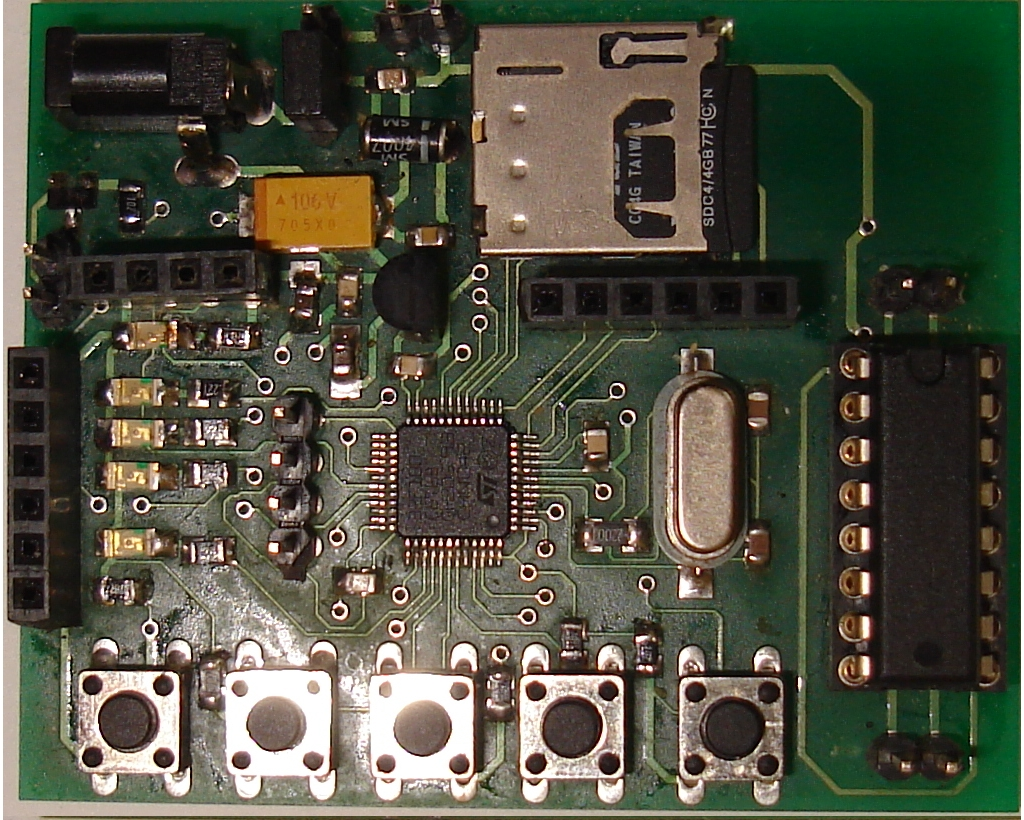
\includegraphics[width=7cm]{test_board.jpg}
\caption{Foto hotovej dosky}
\label{picture1}
\end{figure}

\section{Záver}
 Popísaná realizácia multitaskingu je principiálne použiteľná na akomkoľvek mikrokontroléri. Ukazuje možnosť využiť
mikroprocesor na plný výkon a minimalizovať dobu aktívneho čakania. Vďaka jednoduchosti a otvorenému riešeniu ponúka
priestor pre experimentovanie. Rovnako umožnuje pochopiť fungovanie jadra systému a programovať ďalšie časti, napr. 
semafóry, systém správ alebo ovládače. Možnosti inovácií sú najmä vo voľbe plánovacieho algoritmu, kde sa ponúkajú aj
praktické merania výkonnosti systému, času potrebného na prepnutie kontextu a náročnosti jadra na pamäť.

%============================================================================%
%                                references                                  %
%============================================================================%
\begin{thebibliography}{9}
\bibitem{stm32f}
{\it \url{http://www.st.com/internet/mcu/class/1734.jsp} Vyrobca rady stm32f}
\bibitem{stellaris}
{\it \url{http://www.ti.com/ww/en/embedded/stellaris} Texas Instruments stellaris mikrokontroléry}
\bibitem{armarch}
{\it \url{http://www.root.cz/clanky/mikroprocesory-s-architekturou-arm} arm architektúra}
\bibitem{eventprog}
{\it \url{http://students.cs.byu.edu/~cs124ta/references/HowTos/HowTo_EventDriven.html} ukážka udalosťami riadeného programovania na mikrokontroléri}
\bibitem{disckit}
{\it \url{http://www.st.com/internet/evalboard/product/250863.jsp} dostupná vývojová doska pre stm32}
\bibitem{sources}
{\it \url{https://github.com/michalnand/cortex_m3_os} odkaz na stiahnutie operačného systému}
\end{thebibliography}



\end{document}
%%%%%%%%%%%%%%%%%%%%%%%%%%%%%%%%%%%%%%%%%%%%%%%%%%%%%%%%%%%%%%%%%%

